\documentclass[12pt, oneside]{article}
\usepackage{geometry}
\geometry{letterpaper}
\usepackage{graphicx}
\usepackage{amssymb}
\usepackage{hyperref}
\usepackage{algorithm}
\usepackage{algorithmic}
\graphicspath{{./images/}}
\usepackage{mathtools}
\usepackage{amsmath}
\usepackage[backend=biber, style=numeric]{biblatex}
\DeclarePairedDelimiter\ceil{\lceil}{\rceil}
\DeclarePairedDelimiter\floor{\lfloor}{\rfloor}
\usepackage{pgfplots}
\pgfplotsset{width=10cm,compat=1.9}
\addbibresource{planrefs.bib}

\begin{document}

\title{Location-Based Species Presence Prediction}
\author{Michael Ward \\ tue97607@temple.edu}
\date{April 28, 2022}
\maketitle
\thispagestyle{empty}

\newpage
\pagenumbering{roman}
\tableofcontents
\newpage
\pagenumbering{arabic}

\section{Abstract}
\label{Abstract}

\begin{normalsize}

This paper 

\end{normalsize}
\newpage

\section{Introduction}
\label{Introduction}

\begin{normalsize}

\subsection{Background}

Distribution and diversity of plant and animal species have both always varied in space and time. However, the rise in human population and activities in the last few centuries have drastically impacted the speed and magnitude of change in species distribution and diversity \cite{pinto2021predicting}. Understanding where different species live is crucial to making well-informed conservation decisions. The rapid change in distribution and diversity of species has made the process of conservation decision making harder, since species location data quickly loses its value over time. While humans have caused major disruptions in the distribution and diversity of species, we also generate millions of geo-referenced species observations every year through the work of citizen science projects, which can be used to build species distribution models (commonly referred to as SDM) \cite{lorieul2021overview}.

	The aim of this project is to address the need for predictive species distributions with models based on geo-localized observations of plant and animal species from France and the United States. The task is to return a set of 30 candidate species that should contain the true observed species when provided with a GPS position and its associated features. This work is relevant to the aforementioned fields of biodiversity management and conservation. Specifically, this type of SDM could allow for biodiversity inventories via the development of location-based recommendation services, and accelerate the recording and validation of species observations for the purposes of creating of large-scale and high-quality data sets. Ultimately, the desire is to be able to predict what types of species might be found at a new location, which can be used for the purpose of conservation decision-making.

This project has an associated \href{https://www.kaggle.com/c/geolifeclef-2022-lifeclef-2022-fgvc9/overview}{Kaggle competition}. The competition is held jointly as part of the \href{https://www.imageclef.org/LifeCLEF2022}{LifeCLEF 2022 lab} and \href{https://sites.google.com/view/fgvc9}{FGVC9 workshop}. While this has been an ongoing yearly competition since 2018, there is still considerable room for improvement for this problem. The evaluation metric for this problem is the top-30 error rate, which will be discussed further in section 2.3. I am submitting my work on this project to the Kaggle competition, so I will be evaluating my models according to the top-30 error rate metric that will be used in the competition to evaluate model performance.

The winning solution in 2021 for GeoLifeClef still had a very high top-30 error rate, near 75\%, and was not able to make use of all of the covariate data available. According to an overview of the 2021 competition results, the main challenges associated with this problem have to do with properly aggregating the different covariates, and determining how much complementary or redundant information is contained in the high resolution patches compared to the ones captured from the bioclimatic and soil variables \cite{lorieul2021overview}. I intend to survey current and past research on species prediction to inform my testing of multiple different models that attempt to solve this problem. 

\subsection{Data Description and Visualization}

\subsubsection{Observations}

The dataset contains roughly 1.6 million observations of plant and animal species. There are about 17,000 species in the dataset, 9,000 of which are plant species, while the other 8,000 are animal species. Each observation contains the species name and the gps coordiantes where it was observed. Each observation is also paired with a set of covariates which contain characteristics of the surrounding landscape and environment. The covariates are in tabular, .TIFF, .JPEG, and .GeoTIFF format, and are a combination of high resolution remote sensing imagery, land cover data, altitude, as well as low-resolution climate and soil variables. The observations in this dataset are heavily imbalanced. As seen in Figure 1, the minimum number of observations per class is 3, while the max number of observations per class is 6,701. Additionally shown below in Figure 2 is a graph illustrating the imbalance on a logarithmic scale to emphasize how many classes can be considered as minority classes in this dataset. Over 30\% of the 17,037 classes have just 10 observations or less, out of the roughly 1.6 million total observations.

\begin{figure}[H]
\caption{Dataset Metrics}
\centering
\setlength{\tabcolsep}{0.5em} % for the horizontal padding
{\renewcommand{\arraystretch}{1.2}% for the vertical padding
\begin{tabular}{ |l|r| }
\hline
 Number of Classes (Unique Species) & 17,037 \\
 \hline
 Number of Observations (Training) & 1,627,475 \\  
 \hline
 Number of Observations (Validation) & 40,080 \\
 \hline
 Number of Observations (Testing) & 36,421 \\
 \hline
 Max Number of Observations per Class & 6,701 \\
 \hline
 Min Number of Observations per Class & 3 \\
 \hline
\end{tabular}
}
\end{figure}

\begin{figure}[H]
\caption{observation distribution}
\centering
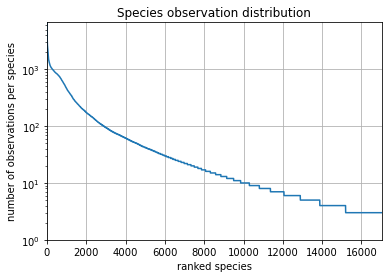
\includegraphics[width=0.8\textwidth]{observations}
\end{figure}

The observations in this data set have been recorded both from the United States and from France. Shown below are the spatial distributions of observations in each country.

\begin{figure}[H]
\caption{US spatial distribution}
\centering
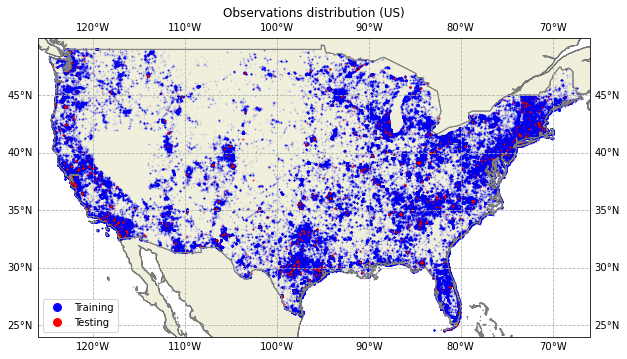
\includegraphics[width=0.7\textwidth]{us_dist}
\end{figure}

\begin{figure}[H]
\caption{FR spatial distribution}
\centering
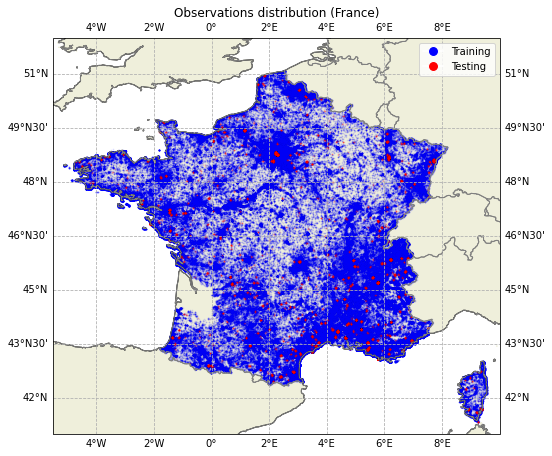
\includegraphics[width=0.7\textwidth]{fr_dist}
\end{figure}

The train/test split for the data has already been determined by the competition, and uses a spatial block holdout procedure to split the data. The reasoning for using a spatial block holdout is to limit the effects of spatial auto-correlation on the data. The way this splitting procedure works is by assigning observations to a grid of 5km by 5km quadrants, of which 2.5\% are randomly sampled to create the test set, another 2.5\% randomly sampled to create the validation set, and the remaining are used for the training set. The validation set is created using the same spatial block holdout procedure \cite{lorieul2021overview}.

\subsubsection{Environmental Vectors}

The main group of data provided by GeoLifeClef is made up of environmental vectors (of which there are 27). These environmental vectors were sourced from two separate databases, WorldClim and SoilGrids. WorldClim is a database containing high spatial resolution global weather and climate data \cite{hijmans2005very}. 19 of the 27 environmental vectors provided by GeoLifeClef are sourced from WorldClim, and mostly includes various Bio-Climatic variables related to temperature and precipitation. SoilGrids is another database of global digital soil mapping that uses machine learning methods to map the spatial distribution of soil properties around the world \cite{hengl2017soilgrids250m}. The 19 bio-climatic variables sourced from WorldClim were extracted from satellite raster imagery with a spatial resolution of 1km\textsuperscript{2}/pixel. The 8 pedologic (soil) variables were extracted from satellite raster imagery with a spatial resolution of 250m\textsuperscript{2}/pixel \cite{lorieul2021overview}.

\begin{figure}[H]
\caption{Environmental Vectors}
\centering
\begin{tabular}{ |l|l| }
\hline
\multicolumn{2}{|c|}{Bio-Climatic Variables (WorldClim) \cite{hijmans2005very}}\\
\hline
Name & Description \\
\hline
bio\_1 & Annual Mean Temperature \\
bio\_2 & Mean Diurnal Range (Mean of monthly (max temp - min temp)) \\
bio\_3 & Isothermality (bio\_2/bio\_7) (* 100) \\
bio\_4 & Temperature Seasonality (standard deviation *100) \\
bio\_5 & Max Temperature of Warmest Month \\
bio\_6 & Min Temperature of Coldest Month \\
bio\_7 & Temperature Annual Range (bio\_5-bio\_6) \\
bio\_8 & Mean Temperature of Wettest Quarter \\
bio\_9 & Mean Temperature of Driest Quarter \\
bio\_10 & Mean Temperature of Warmest Quarter \\
bio\_11 & Mean Temperature of Coldest Quarter \\
bio\_12 & Annual Precipitation \\
bio\_13 & Precipitation of Wettest Month \\
bio\_14 & Precipitation of Driest Month \\
bio\_15 & Precipitation Seasonality (Coefficient of Variation) \\
bio\_16 & Precipitation of Wettest Quarter \\
bio\_17 & Precipitation of Driest Quarter \\
bio\_18 & Precipitation of Warmest Quarter \\
bio\_19 & Precipitation of Coldest Quarter \\
\hline
\multicolumn{2}{|c|}{Pedologic Variables (SoilGrids) \cite{hengl2017soilgrids250m}} \\
\hline
Name & Description \\
\hline
orcdrc & Soil organic carbon content (g/kg at 15cm depth) \\
phihox & Ph x 10 in H20 (at 15cm depth) \\
cecsol & cation exchange capacity of soil in cmolc/kg 15cm depth \\
bdticm & Absolute depth to bedrock in cm \\
clyppt & Clay (0-2 micro meter) mass fraction at 15cm depth \\
sltppt & Silt mass fraction at 15cm depth \\
sndppt & Sand mass fraction at 15cm depth \\
bldfie & Bulk density in kg/m3 at 15cm depth \\
 \hline
\end{tabular}
\end{figure}

\subsubsection{Satellite Imagery}

Each observation in the dataset has 4 associated high resolution satellite images, one covering the rgb spectrum, one covering the near infrared spectrum (NIR), one with altitude measurements, and one with land cover classifications. Each image are a spatial resolution of 1 meter per pixel, and are 256 x 256 pixels (256 meters x 256 meters). Each image is centered on it's associated observation. The United States RGB and NIR images were sourced from the 2009 to 2011 cycle of the National Agriculture Imagery Program (NAIP), while the French RGB and NIR images are sourced from the BD-ORTH 2.0 and ORTHO-HR 1.0 databases from the Institut national de l'information géographique et forestière. The United States land cover imagery that is used in this dataset is sourced from the National Land Cover Database, and the French land cover imagery is sourced from the Centre d'Etudes Spatiales de la Biosphère \cite{homer2015completion}. The elevation imagery is sourced from the NASA Shuttle Radar Topography Mission for both the US and French observations. Below is an example of the satellite raster imagery available for an observation.

\begin{figure}[H]
\caption{Satellite Raster Imagery}
\centering
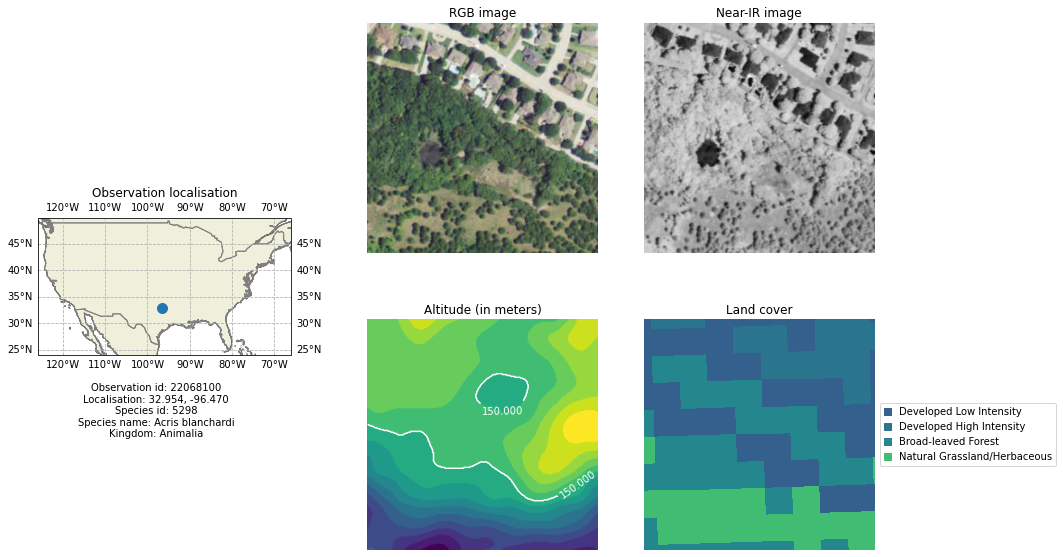
\includegraphics[width=1\textwidth]{raster}
\end{figure}

\subsection{Accuracy Evaluation}

The main metric that I will use to evaluate my models is the top-30 error rate, which is a set-valued classification metric defined by the Kaggle competition. Each observation $i$ in the dataset is associated with a single ground-truth label $y_{i}$ which corresponds to the observed species. The model must provide 30 candidate labels $\hat{y}_{i,1},\hat{y}_{i,2}, ... , \hat{y}_{i,30}$ for each observation. The top 30 error rate is then computed using the following equation:

\[ 
\textnormal{Top-30 error rate = } \ \frac{1}{N} \sum\limits_{i=1}^N e_{i} \ \ \textnormal{where} \ \ e_{i} = 
\bigg\{
	  \begin{tabular}{l}
	  1 \ \ \textnormal{if} $\forall k \in$ \big\{1, ... , 30\big\}, $\hat{y}_{i,k} \neq y_{i}$ \\
	  0 \ \ \textnormal{otherwise} \\
	  \end{tabular}
\] 

There are several reasons to use this type of error measure as the main evaluation metric for this problem and data. The first reason being that this data set contains presence-only observations, meaning that each observation only contains the presence of one species whilst many different species could potentially be recorded from each geographic location. A set-valued classification metric allows for more precision when measuring the accuracy of predicted sets when dealing with the limited knowledge inherent with presence-only observations. Second, recent research has shown that using single-output predictions for ambiguous multi-class datasets leads to overall poor performance and results \cite{chzhen2021set}. For a dataset such as this with over 17,000 classes and many classes with as few as 3 observations, it makes sense to use a more lenient set-valued classification metric which allows for more meaningful comparison of models and input data types, instead of a single-output prediction per observation.

\end{normalsize}

\section{Related Work}
\label{Related Work}

\begin{normalsize}

\subsection{Mapping Species Distributions}

The most widely cited resource when it comes to the general topic of species distribution modeling is a 2017 textbook named Mapping Species Distributions by Janet Franklin. This text is a comprehensive overview on the topic of species distribution modeling, covering not just the models used within the field, but also the history and ecological basis of species distribution modeling. This text breaks the SDM methods into two broad categories of statistical methods, and machine learning based methods. Among the statistical methods discussed in this text are generalized linear models (GLM), generalized additive models (GAM), and multivariate adaptive regression splines (MARS). 

This text identifies generalized linear modeling as the most established / most generally accepted statistical framework for SDM.  Their reasoning for the popularity of GLM in SDM is the ability of the link function to handle response variables with irregular distributions. Overall, the author is critical of the statistical approaches to SDM due to their assumption that observations are independent. These approaches violate Tobler's 'First Lax of Geography', that near things tend to be similar to each other due to the fact that they are likely to influence each other or be influenced by the same local environmental factors \cite{franklin2010mapping}. I am in agreement with the author that this law of geography should not be ignored when working with spatial data.

Franklin also covers the most commonly used machine learning techniques used for SDM at the time, which are identified broadly as  ensemble methods, deep learning methods, and genetic algorithms. Out of these categories, the methods that have been most widely successful in the field of ecology and for the purposes of SDM are random forests and other ensemble methods such as stochastic gradient boosting, various flavors of neural networks, and support vector machines. Ensemble methods are identified as the most applied method, due to their great success with complex classification problems. While neural networks and SVM have also shown promise in this field, the author shows evidence that while these methods have performed well on complex classification problems, they sometimes performed worse or no better than statistical methods like GLMs or GANs, or ensemble methods like random forests. In addition to this, neural networks have a steep learning curve to be used effectively which has resulted in a slower adoption in the field of ecology compared to other machine learning based methods \cite{franklin2010mapping}.

\subsection{Review of Machine Learning Based SDM}

Another 2017 publication talks in more detail about the specific benefits and flaws of several machine learning techniques with respect to their usage in species distribution modeling.  These authors surveyed 258 journal and conference papers published between 2000 and 2017 that contained both 'machine learning' and 'species' distribution' to determine what the most common machine learning methods in SDM are today. In this paper, the authors compare random forests, MaxEnt, support vector machines, and artificial neural networks. These four methods are not exhaustive, but comprise the four most widely used methods out of the surveyed material. 

The authors provide an overview of cases where these methods were applied, and give their thoughts on the usage of each method. First, the authors highlight the importance of combining these methods with expert domain knowledge: their research found that the usefulness of these machine learning methods are highly dependent on the ecological assumptions that influenced the choice of environmental variables used. Ultimately, the ideal relationship should be one where ecologists focus on ecological explainability, while data scientists focus on predictive performance.

In terms of model evaluation in SDM, the authors group random forests, MaxEnt, and SVM together as ensemble methods and compare them to the usage of deep learning. The authors find that ensemble methods are the most widely applied methods in SDM, and have achieved considerable results. In comparison, deep learning methods have been slower to adopt in the ecology field, though the authors have found successful application of deep learning models in tree species classification, plant disease detection, and plant phenotyping. They cite three reasons for deep learning having less prevalence in the field of ecology, comparatively to ensemble methods; First, they agree with Franklin that deep learning is more difficult and time consuming for ecologists to learn and master. Additionally, it is less preferred due to its lack of ecological interpretability. Lastly, the hardware or cloud platforms necessary for supporting deep learning when working with large amounts of raster data is quite expensive. Despite these reasons for deep learning's lack of current usage in SDM and ecology, the authors believe that adoption will increase over time due to the increase of software platforms that support deep learning, and the possibility of deep neural networks performing better than ensemble methods on larger and more complex data sets \cite{8328619}.


\subsection{Predicting Rare Species Distributions}

One of the underlying issues of SDMs has to do with generalizing species distributions in large undersampled areas, especially with few observations available \cite{mi2017choose}. This is certainly a problem for this project, as over 30\% of the \~17,000 species have 10 observations or less, and the spatial distribution of observations is not consistent across either the United States or France. One paper has assessed what methods can best address this underlying issue of SDMs by testing multiple machine learning models on three case studies containing rare species distributions in China \cite{mi2017choose}. Other research, such as the papers and textbooks previously mentioned, has proved the effectiveness of machine learning techniques in ecology and SDM, but has not tested which methods perform best with imbalanced observations and rare classes \cite{cutler2007random}.

Chunrong Mi et al. quantify which models out of stochastic gradient bossting, random forest, CART, and MaxEnt, perform best on three separate cases of rare species distribution in China (Hooded Crane with 33 observations, White Naped Crane with 40 observations, and Black Necked Crane with 75 observations) \cite{mi2017choose}. This study was most relevant to my methodology out of the other literature found due to both the addressing of rare species distribution, and the usage of WorldClim environmental vectors for the predictive variables. Chunrong Mi et al. used WorldClim variables bio\_1 through bio\_15 in addition to several variables obtained from naturalearthdata.com which provides distance to relevant land and water features for their predictive variables. This was relevant, as I am using WorldClim variables bio\_1 through bio\_19 in my models.

The authors found that random forests had the best performance in predicting the distribution of each of the three rare crane species by a significant amount, using area under ROC curve and the true skill statistic as accuracy metrics. The authors also comment that the application of a few observations to project a distribution area beyond its sampled range is a large challenge that hasn't been attempted until recently in ecology and SDM. Because of this, they recommend that modelers should assess their model performance on not just an evaluation metric (such as AUC or TSS), but also combine the use of visualization and expert domain knowledge to assess how the predicted species distribution map looks and compares to real data \cite{mi2017choose}.

\end{normalsize}

\section{Methodology}
\label{Methodology}

\begin{normalsize}

\subsection{Missing Data}

Roughly 3.6\% of observations are missing data for the soil variables sourced from SoilGrids, and roughly 2.6\% of observations are missing data for the geo-climatic variables sourced from WorldClim. Before making any decisions on how to handle the missing data I plotted a missingness graph to see how much data was missing, and whether there were correlations in the missing data.

\begin{figure}[H]
\caption{Missingness Plot}
\centering
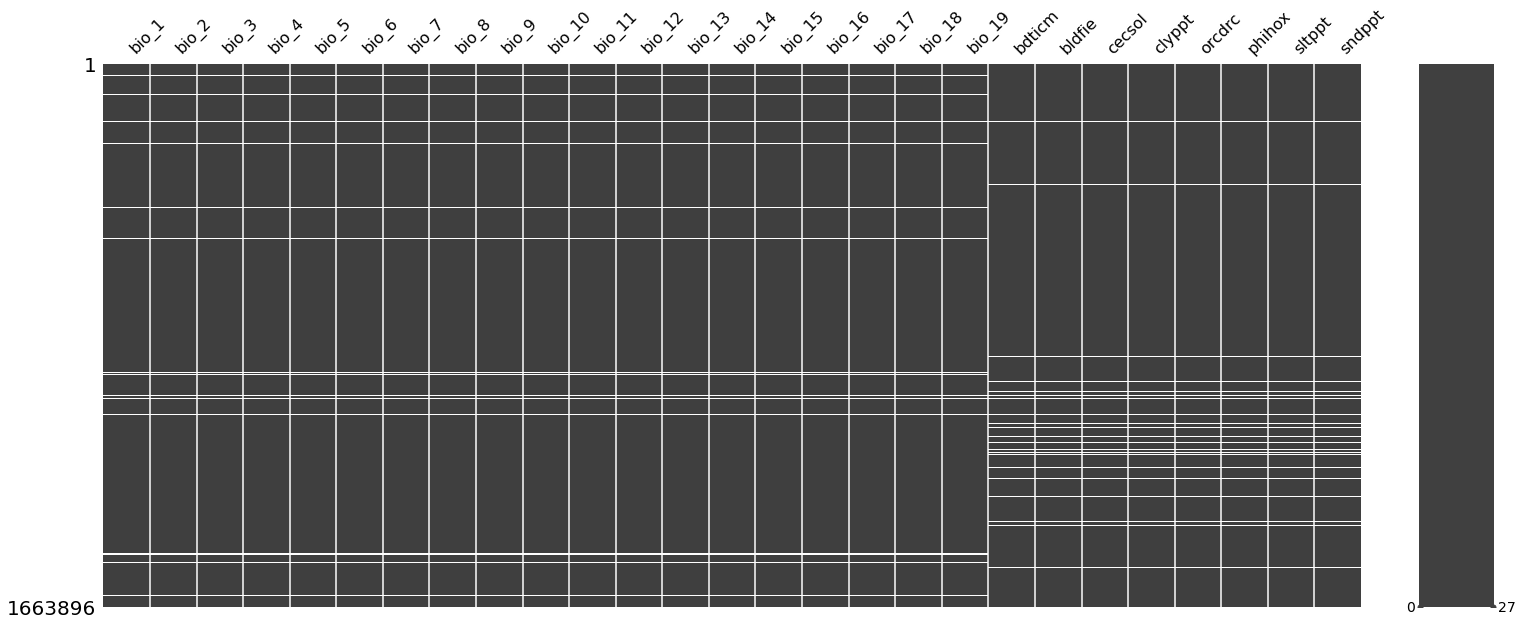
\includegraphics[width=0.9\textwidth]{missingno}
\end{figure}

The missingness plot above shows which variables are missing data on the x-axis, and shows the position in the data set in which they are missing on the y-axis. If a line runs straight across the x-axis, that means that there is a correlation in the missing data, and it should not be considered missing at random. In this case, you can see that all of the missing data is either correlated to WorldClim or SoilGrid - if an observation is missing one WorldClim variable it is missing all WorldClim variables. Likewise, if an observation is missing one SoilGrid variable, it is missing all other SoilGrid variables. A small portion of missing data (roughly 1\%) is 100\% correlated, meaning that it is missing all variables. 

Since the missing data is missing not at random and many minority classes have less than 10 observations, it is not appropriate to drop the missing rows of data in this case. I decided to test my models with two different methods of imputation. The first method of imputation I used was a form of simple imputation, where the mean value of a variable is imputed for that variable's missing values. The second form of imputation I tested was k-nearest neighbors imputation, where each missing value is imputed using the mean value of that observation's k-nearest neighbors. I used a value of 20 for k for imputation.

\subsection{Baseline}

In order to have a baseline to compare my model results to, besides other competitors in the Kaggle competition, I went with a relatively simple baseline that makes sense for the dataset that I am working with. As a reminder, the top-30 error rate metric requires 30 species to be predicted for each observation in the dataset. I created a baseline that just estimates the top-30 most present species in the dataset for each observation. This baseline has a top-30 error rate of 93.5\%.

\subsection{Modeling}

\subsubsection{KNN}

One machine learning classifier that I hadn't seen come up frequently during my review of related literature is the k-nearest neighbors classifier. I decided to give this classifier a try to see how it would compare specifically to random forests on this data. While testing KNN, I iteratively increased K until it reached diminishing returns on the top 30 error rate. After reaching the rate of diminishing returns, I used grid search with 5 fold cross validation to tune the KNN hyper parameters. I specifically tested different distance metrics, prediction weights, and the KNN algorithm used to compute nearest neighbors (KDTree, BallTree, and brute force search). I ran each of the KNN models using all 27 environmental variables as features.

\subsubsection{Random Forests}

The second classification method I used in my methodology was random forests. All of the literature I reviewed pointed to random forests as the best technique for species distribution modeling, especially when working with rare and sparse species. For this method I also used grid search with 5 fold cross validation to tune the hyper parameters of the model and test multiple iterations. The specific parameters that I tested were differing numbers of trees per forest, the splitting criterion used (gini vs. entropy), and the maximum tree depth allowed. I also ran the random forest models using all 27 environmental variables as features.

\subsubsection{Deep Neural Network}

The last classification method that I wanted to use in my experiment was a deep neural network, though I ran into several roadblocks while attempting to test this method. My intention was to use a convolutional neural network with the 


\end{normalsize}

\section{Discussion}
\label{Discussion}

\begin{normalsize}

\subsection{Results}

\subsubsection{KNN Results}

\subsubsection{Random Forests Results}

\subsubsection{Comparison}

\subsection{Limitations}

\end{normalsize}

\section{Acknowledgments}
\label{Acknowledgments}

\begin{normalsize}

I would like to thank the contributors and maintainers of the GeoLifeCLEF Github repository: Maxi Miliense, Titouan Lorieul, Benjamin Deneu, Chris Botella, and Elijah Cole. This repository contains open source Python code that was designed for GeoLifeCLEF Kaggle challenge competitors, specifically for loading, plotting, and submitting the data provided in the competition. This code was especially useful for me to get up and running quickly with loading and visualizing the data, so I could move on to transforming the data and running models. I used the provided python functions for spatially plotting data, and generating the competition submission files. I would also like to thank Temple's CIS 4523/5523 Professor Zoran Obradovic and teaching assistant Marija Stanojevic for providing valuable feedback on this project during project presentations.

\end{normalsize}

\section{References}
\label{References}
\nocite{*}
\printbibliography[heading=none]

\end{document}